\section{Covariance, dérivées et prévisions de Fisher}
\label{sec:framework}
% =====================================================================

Pour prévoir avec quelle précision une statistique contraint les paramètres cosmologiques, deux ingrédients sont nécessaires : de combien la statistique fluctue d'une réalisation de l'Univers à l'autre à paramètres fixés, sa \emph{covariance}, et de combien elle change quand un paramètre change, ses \emph{dérivées}. Une statistique est informative si sa réponse aux paramètres est grande devant ses fluctuations. La matrice de Fisher combine les deux (Section~\ref{sec:fishermat}). Cette section explique comment nous avons obtenu chaque ingrédient, et pourquoi chacun a exigé un jeu de données dédié.

\paragraph{Vecteurs de données.} Par défaut, les corrélations croisées des quartiles extrêmes Q1 et Q4 avec les galaxies, $\ell=0,2$, $20\le s\le150\Mpch$ en bins de $10\Mpch$ (13 bins par multipôle, 52 nombres par méthode), avec ou sans la 2PCF (26 nombres). Des variantes ajoutent les auto-corrélations des quartiles, utilisent les quartiles de galaxies, des quartiles isolés, ou changent l'échelle minimale.

\subsection{Covariance}

La covariance fixe les barres d'erreur des prévisions et les corrélations entre les bins et les statistiques d'un vecteur de données. Elle doit être estimée à partir de nombreuses réalisations indépendantes du même modèle, mesurées exactement comme les données. \paragraph{Référence : 1786 boîtes indépendantes.} La covariance est mesurée sur les 1786 petites boîtes officielles (Section~\ref{sec:official}) : 1786 volumes indépendants de $(500\Mpch)^3$ traités exactement comme nos sous-volumes. Les prévisions sont données pour ce volume de $0.125\,(h^{-1}{\rm Gpc})^3$. La matrice de corrélation (Figure~\ref{fig:corr}) montre de fortes corrélations entre échelles voisines, entre les corrélations croisées Q4 et la 2PCF, et des anti-corrélations entre les blocs Q1 et Q4. Les blocs ASTRA et density split d'un même quartile sont très fortement corrélés : étant mesurés sur les mêmes galaxies, leur bruit est largement commun. C'est l'origine de leur complémentarité : lorsque deux mesures partagent la majeure partie de leur bruit mais répondent différemment aux paramètres, leur combinaison annule une partie de ce bruit et gagne bien plus que des mesures indépendantes.

\paragraph{Première approche : 192 sous-volumes d'une boîte.} Avant l'usage des mocks officiels, la covariance était estimée à partir du catalogue fiduciel de la suite d'émulation (\texttt{c000}, \texttt{hod239}, le tirage de c000 le plus proche du centre du prior de HOD), en utilisant les 64 sous-volumes mesurés selon les trois lignes de visée, soit $N_s=192$ échantillons. Les trois lignes de visée ne sont pas indépendantes, approximation couramment utilisée dans les analyses fondées sur des simulations. L'inverse de la covariance est corrigé par le facteur de Hartlap \cite{Hartlap2007} (Annexe~\ref{app:maths}), $(N_s-N_d-2)/(N_s-1)$ : 0.72 pour une méthode ($N_d=52$), 0.59 avec la 2PCF ($N_d=78$), 0.31 pour ASTRA + DS + 2PCF ($N_d=130$), ce qui a motivé la compression des vecteurs de données (Section~\ref{sec:fishermat}). La Section~\ref{sec:choices} montre comment le remplacement de cette covariance par la covariance indépendante a modifié la comparaison.

\begin{figure}[!htbp]
\centering
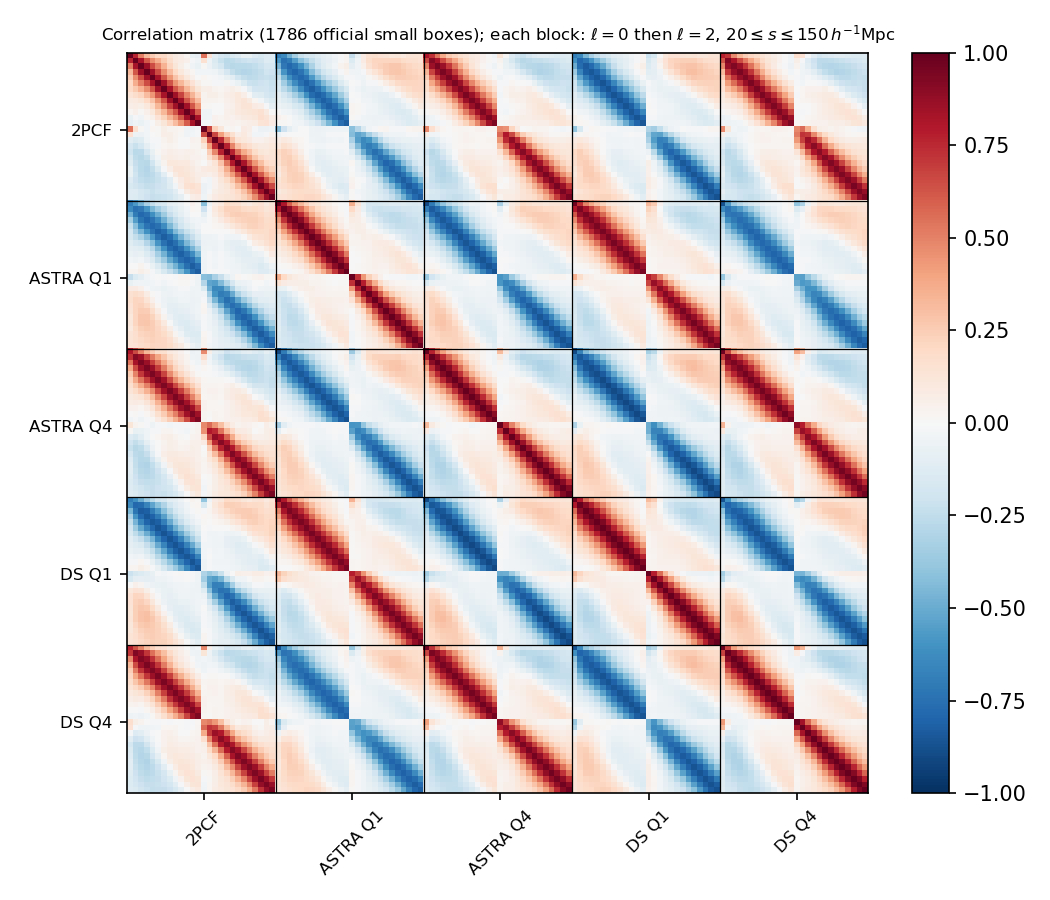
\includegraphics[width=\linewidth]{v2_corr.png}
\caption{Matrice de corrélation de la 2PCF et des corrélations croisées Q1, Q4 de l'ASTRA split et du density split (1786 petites boîtes officielles).}
\label{fig:corr}
\end{figure}

\subsection{Différences finies : le problème de la discordance de HOD}
\label{sec:finitediff}

La grille de dérivées d'AbacusSummit fournit, pour chaque paramètre, deux simulations ne différant que par un petit changement de ce paramètre et partageant les mêmes conditions initiales. Une estimation naturelle des dérivées est la différence finie appariée : pour chaque paramètre, nous sélectionnons un fichier de HOD dans chaque cosmologie de la paire, en minimisant la distance entre les deux vecteurs de paramètres de HOD (Tableau~\ref{tab:hods}), et nous différencions les statistiques sous-volume par sous-volume et ligne de visée par ligne de visée avant de moyenner, de sorte que la variance cosmique commune aux deux simulations s'annule en grande partie. Cette annulation n'est que partielle : chaque catalogue de HOD est un tirage indépendant des galaxies peuplant les halos, donc le bruit d'échantillonnage des galaxies n'est pas partagé, et la différence de deux mesures sur boîte entière avec des HOD différentes a une erreur comparable à celle d'une seule boîte (1.05 fois, médiane sur les paires de la grille). La précision des dérivées appariées vient de la moyenne sur les 192 échantillons appariés.

\begin{table}[!htbp]
\centering\small
\begin{adjustbox}{max width=\linewidth}
\begin{tabular}{lccc}
\toprule
Paramètre & Fichiers de HOD & $|\Delta h|$ & paires aléatoires \\
\midrule
fiducielle & c000\_hod239 & -- & -- \\
$\omega_b$ & c100\_hod448 / c101\_hod694 & 0.63 & 1.38 \\
$\omega_{\rm cdm}$ & c102\_hod589 / c103\_hod841 & 0.58 & 1.38 \\
$n_s$ & c104\_hod308 / c105\_hod735 & 0.65 & 1.37 \\
$\sigma_8$ & c112\_hod230 / c113\_hod204 & 0.65 & 1.39 \\
\bottomrule
\end{tabular}
\end{adjustbox}
\caption{Catalogues de HOD des paires de différences finies. $|\Delta h|$ est la distance entre les deux vecteurs de paramètres de HOD normalisée à l'étendue du prior (12 paramètres) ; la dernière colonne donne la médiane pour des paires aléatoires.}
\label{tab:hods}
\end{table}

Moyennées sur les 192 échantillons, ces différences ont de faibles erreurs statistiques, mais ce ne sont pas des dérivées cosmologiques, et c'est l'un des principaux résultats de ce travail. Une différence de paire est la somme de deux termes : le terme cosmologique, le changement des statistiques dû au paramètre (la physique), et le terme de HOD, le changement dû aux connexions galaxie--halo différentes des deux catalogues (un changement du modèle de formation des galaxies du mock, non de la cosmologie). Nous avons estimé le terme de HOD à partir de 72 catalogues supplémentaires de la cosmologie fiducielle avec des HOD différentes, qui donnent la réponse des statistiques à chaque paramètre de HOD, évaluée à la différence de HOD de chaque paire, et nous l'avons comparé, en unités de l'erreur statistique, au terme cosmologique prédit à HOD fixée : le terme de HOD est 10 à 15 fois plus grand. Les vecteurs de dérivées par rapport à $\omega_b$, $n_s$ et $\sigma_8$ sont alors presque colinéaires (corrélations 0.95--0.99 dans la métrique de Fisher), car ils mesurent tous principalement la même réponse à la HOD, et les matrices de Fisher ne sont pas définies positives. Nous avons essayé de soustraire le terme de HOD : un modèle linéaire de la réponse à la HOD prédit des catalogues exclus avec une erreur de 45\%, un modèle à processus gaussien (un GP par composante principale du vecteur de données, noyau anisotrope) avec 8\%. Mais une correction erronée de 8\% sur un terme dix fois plus grand que le signal laisse un résidu de $0.08\times10\simeq0.8$ fois le signal : les dérivées corrigées restent dominées par l'erreur de la correction, et les matrices de Fisher restent instables. Toute suite d'émulation dans laquelle la HOD est tirée indépendamment dans chaque cosmologie a ce problème.

Ces différences finies restent utiles de trois façons. Premièrement, elles mesurent le problème : elles montrent de combien le terme de HOD domine, ce qui nous apprend que toute dérivée issue d'une telle suite doit être prise à HOD fixée. Deuxièmement, une fois corrigées du terme de HOD avec le processus gaussien, elles donnent des dérivées qui n'impliquent aucun réseau de neurones, avec lesquelles l'émulateur peut être vérifié (Figure~\ref{fig:emu_pairs}). Troisièmement, avec plusieurs tirages de HOD dans chaque cosmologie de la grille de dérivées, elles deviennent une régression qui estime les dérivées exactement à la HOD fiducielle (Section~\ref{sec:regression}).

\subsection{Émulateur par réseau de neurones}
\label{sec:emulator}

\paragraph{Pourquoi un émulateur.} Comme dans SUNBIRD \cite{CuestaLazaro2024}, nous modélisons chaque statistique comme une fonction lisse des paramètres cosmologiques et de HOD, et nous prenons ses dérivées à HOD exactement fixée par différentiation automatique, ce qui supprime par construction la discordance de HOD.

\paragraph{Entrées et sorties.} Les entrées sont les 8 paramètres cosmologiques variés dans AbacusSummit ($\omega_b$, $\omega_{\rm cdm}$, $\sigma_8$, $n_s$, $\alpha_s$, $N_{\rm ur}$, $w_0$, $w_a$ ; $h$ et $A_s$ découlent de $\theta_*$ et $\sigma_8$) et les 12 paramètres de HOD, remis à l'échelle de $[0,1]$ sur le prior. La sortie d'un réseau est une statistique, le monopôle et le quadrupôle pour $20\le s\le150\Mpch$ en bins de $10\Mpch$ (26 nombres), mesurés sur la boîte entière comme la moyenne des 64 sous-volumes, standardisés par leur moyenne et par l'erreur statistique de la boîte entière $\sigma_{\rm box}$. Il y a un réseau par statistique (33 statistiques).

\paragraph{Architecture et entraînement.} Chaque réseau est un perceptron multicouche entièrement connecté : 20 entrées, trois couches cachées de 256 unités et 26 sorties, soit environ $1.4\times10^5$ poids. C'est le type de réseau utilisé par SUNBIRD \cite{CuestaLazaro2024} pour les statistiques de density split ; les sorties sont des fonctions lisses des entrées, que de tels réseaux représentent bien, et la taille est un compromis entre flexibilité et les $\sim1000$ catalogues d'entraînement. Nous n'avons pas exploré systématiquement d'autres architectures ; la courbe d'apprentissage ci-dessous indique que la précision est limitée par le bruit des catalogues d'entraînement plutôt que par le réseau. Nous utilisons des activations SiLU plutôt que les ReLU courantes parce qu'elles sont lisses : les dérivées d'un réseau ReLU sont constantes par morceaux, ce qui rendrait bruitées les dérivées de Fisher. Les réseaux sont entraînés avec l'optimiseur Adam, avec arrêt précoce lorsque l'erreur sur les cosmologies de validation cesse de diminuer. Avec la standardisation ci-dessus, la fonction de perte est un $\chi^2$ par bin, de sorte que le réseau est pénalisé proportionnellement à la signification statistique de ses erreurs. Chaque statistique dispose d'un ensemble de 10 réseaux d'initialisations différentes ; la prédiction est la moyenne de l'ensemble, et la dispersion entre membres mesure l'incertitude due à l'entraînement.

\paragraph{Ensemble d'entraînement.} 999 catalogues des 85 cosmologies : 8 tirages de HOD par cosmologie, les 72 catalogues de calibration fiduciels, et 16 tirages proches de la HOD fiducielle dans c000 et dans chacune des 14 cosmologies de la grille de dérivées, où les dérivées sont évaluées (densification, ci-dessous). Les ensembles de validation et de test comptent 8 cosmologies chacun, jamais vues à l'entraînement.

\paragraph{Précision.} Sur les cosmologies de test, l'émulateur reproduit les 33 statistiques avec une erreur médiane de 0.4--0.9 $\sigma_{\rm box}$, l'erreur statistique d'une boîte entière de $2\,h^{-1}$Gpc (Figure~\ref{fig:emu}). Les erreurs sont les plus grandes aux plus petites échelles et dans les monopôles. Ce que cela signifie dépend du volume analysé : c'est environ dix fois moins que l'erreur du volume de $(500\Mpch)^3$ des prévisions, de sorte que pour nos comparaisons l'erreur de l'émulateur est négligeable (elle est néanmoins ajoutée à la covariance) ; pour une boîte entière de $(2\,h^{-1}{\rm Gpc})^3$, elle est comparable à l'erreur statistique, de sorte qu'une analyse d'un tel volume, ou d'un volume de type DESI, serait limitée par l'émulateur. Une courbe d'apprentissage, par réentraînement sur 25, 50, 75 et 100\% de l'ensemble d'entraînement, montre que cette erreur a atteint un plateau à $\simeq0.5\sigma_{\rm box}$, fixé par le bruit d'échantillonnage des galaxies des catalogues individuels : davantage de catalogues du même type n'aideraient guère, et la réduire exige plusieurs réalisations de HOD par point d'entraînement (Annexe~\ref{app:path}).

\paragraph{Réponse cosmologique.} Des prédictions précises ne garantissent pas des dérivées précises. Nous testons ces dernières en entraînant l'émulateur sans les 14 cosmologies de la grille de dérivées et en comparant sa prédiction des différences $\pm$ des paires, discordance de HOD comprise, aux simulations (Figure~\ref{fig:loco}). La réponse à $\sigma_8$ et $n_s$ est reproduite à 10--20\%, la réponse à $\omega_b$ à 30--45\% avec la bonne forme, mais la réponse à $\omega_{\rm cdm}$ n'est pas capturée en dessous de $s\simeq70\Mpch$ : à $\theta_*$ et $\sigma_8$ fixés, son effet est inférieur à l'erreur de l'émulateur et n'est pas appris loin des points d'entraînement. Cela nous a conduits à \emph{densifier} l'ensemble d'entraînement autour du point fiduciel avec les 16 tirages de HOD les plus proches de la HOD fiducielle dans c000 et dans chaque cosmologie de la grille (240 catalogues), de sorte que l'émulateur voie la réponse à chaque paramètre pour de nombreuses connexions galaxie--halo similaires. La densification seule n'a pas stabilisé les dérivées : les erreurs de Fisher des réseaux individuels variaient de 70--170\% pour la 2PCF et pour $\omega_{\rm cdm}$ et $n_s$, et la comparaison ASTRA/density split changeait de signe d'un entraînement à l'autre. Comme vérification indépendante, les dérivées de l'émulateur à HOD fixée s'accordent avec les différences de paires corrigées par GP à 1--3\% pour $n_s$ et $\omega_{\rm cdm}$, 5--6\% pour $\sigma_8$ et 8--13\% pour $\omega_b$ (Figure~\ref{fig:emu_pairs}).

\paragraph{Entraînement sur les différences de catalogues.} Pour contraindre directement la réponse près du point fiduciel, nous ajoutons à la fonction de perte le $\chi^2$ des \emph{différences} prédites entre catalogues, sur 2544 paires : toutes les paires $(c_+,h_i),(c_-,h_j)$ des sept paires $\pm$ de la grille avec des HOD à moins d'une étendue de prior de la fiducielle, et des paires de la même cosmologie (réponse à la HOD) ; détails dans l'Annexe~\ref{app:maths}. Les différences ne sont pas beaucoup plus précises que les mesures individuelles, puisque le bruit d'échantillonnage des galaxies n'est pas partagé, mais le terme contraint leur \emph{structure} : le réseau doit reproduire la façon dont les statistiques changent entre points voisins de l'espace des paramètres, ce qu'exigent les dérivées. Nous avons aussi testé un poids supplémentaire $(25\Mpch/s)^\alpha$, $\alpha=1$, sur les petites échelles. Nous avons validé les trois variantes sur 56 catalogues locaux (4 par cosmologie de la grille) exclus de l'entraînement, en prédisant les différences de toutes les paires $\pm$ exclues (Tableau~\ref{tab:local}, Figure~\ref{fig:local}). Le terme de différences divise l'erreur par deux pour $\omega_b$ et $\sigma_8$ et la réduit pour tous les paramètres sauf $\omega_{\rm cdm}$, déjà reproduit à 11\% près du point fiduciel ; les résidus atteignent le niveau de bruit des différences mesurées ($\simeq1\sigma_{\rm box}$), de sorte que les données ne permettent pas un test plus sévère. Le poids aux petites échelles apporte un gain supplémentaire marginal mais rend instables les prévisions incluant les auto-corrélations des quartiles ; nous utilisons donc le terme de différences sans lui : c'est l'émulateur de référence.

\begin{table}[!htbp]
\centering\small
\begin{adjustbox}{max width=\linewidth}
\begin{tabular}{lccccccc}
\toprule
 & $\omega_b$ & $\omega_{\rm cdm}$ & $n_s$ & $\alpha_s$ & $w_0$ & $w_0,w_a$ & $\sigma_8$ \\
\midrule
sans terme de diff. & 21 & 11 & 35 & 14 & 17 & 17 & 13 \\
terme de diff. & 10 & 11 & 27 & 10 & 12 & 10 & 7 \\
+ petites échelles & 8 & 11 & 26 & 9 & 11 & 8 & 7 \\
\bottomrule
\end{tabular}
\end{adjustbox}
\caption{Erreur relative médiane (\%) de la prédiction par l'émulateur des différences entre catalogues locaux exclus des paires $\pm$ de la grille de dérivées, pour les trois variantes d'entraînement.}
\label{tab:local}
\end{table}

\paragraph{Dérivées.} La Figure~\ref{fig:derivs} montre les dérivées de référence de la 2PCF et des corrélations croisées Q1, Q4, sous la forme du changement de chaque statistique pour un petit changement de chaque paramètre, en unités de l'erreur statistique. Trois caractéristiques comptent pour les prévisions. (i) Les deux méthodes répondent de façon très similaire à $\omega_{\rm cdm}$ et $n_s$, principalement par le monopôle à $s<75\Mpch$ : ces paramètres changent la forme du clustering en fonction de l'échelle. (ii) Les corrélations croisées de Q1 (vides) répondent avec le signe opposé à celui de Q4 et de la 2PCF. Une statistique seule ne peut distinguer un changement de cosmologie d'un changement de biais des galaxies, par exemple, qui change aussi l'amplitude ; deux statistiques qui répondent en sens opposés au paramètre mais dans le même sens au biais le peuvent, et c'est ainsi que les environnements lèvent les dégénérescences. (iii) À HOD fixée, $\sigma_8$ agit principalement sur les quadrupôles, c'est-à-dire par le champ de vitesses. Les Figures~\ref{fig:der_astra} et~\ref{fig:der_ds} montrent la réponse des quatre quartiles : elle est ordonnée de Q1 à Q4 pour $\omega_{\rm cdm}$, $n_s$ et $w_a$, les quartiles extrêmes répondant le plus, alors que les réponses des monopôles à $\sigma_8$ et $w_0$ sont faibles et sans ordre simple.

\begin{figure*}[!tp]
\centering
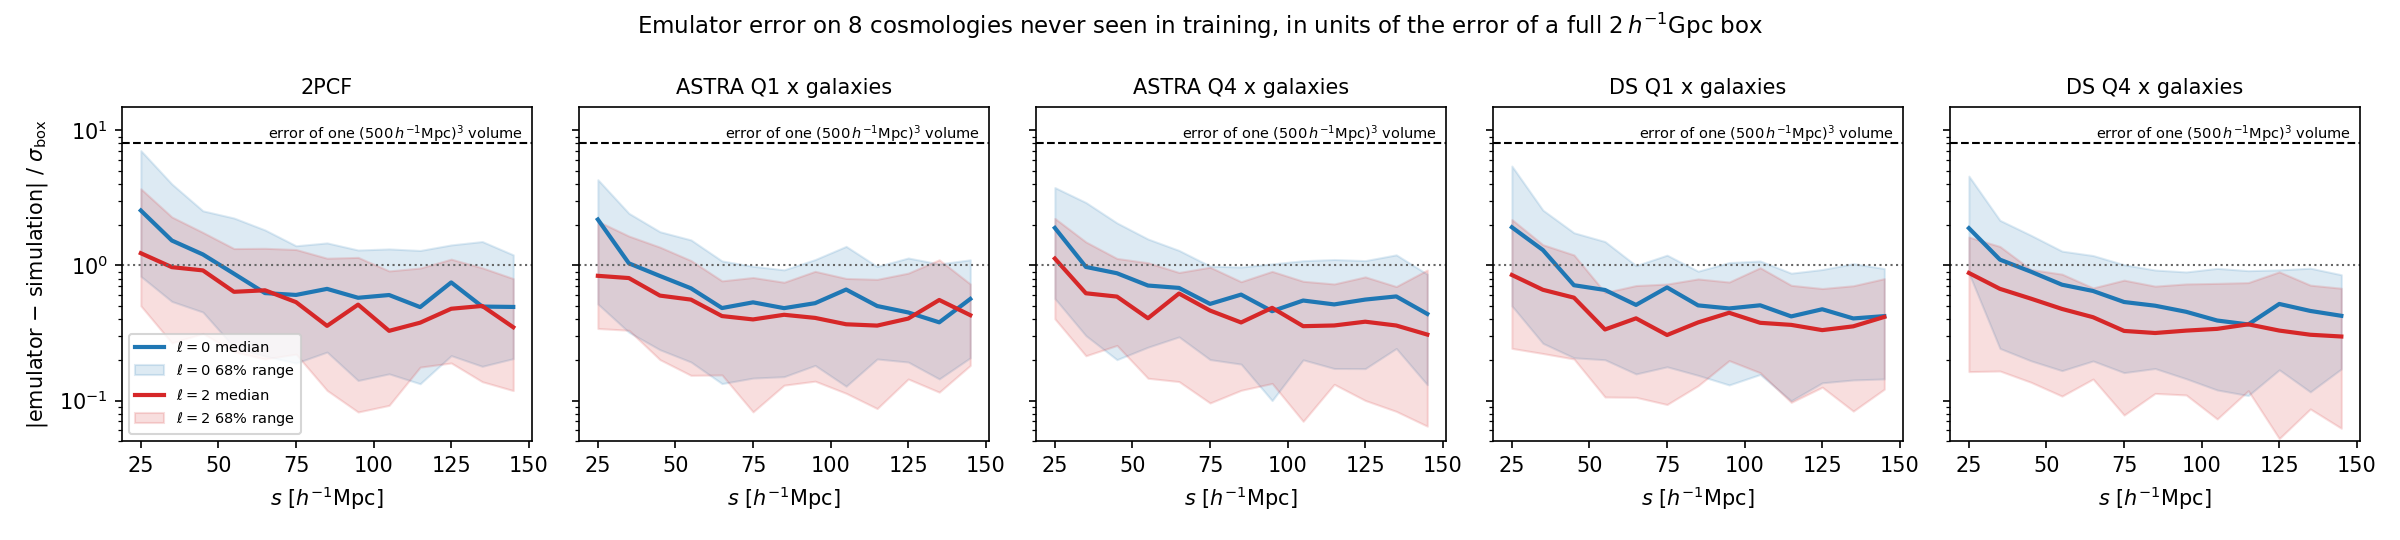
\includegraphics[width=\textwidth]{readable_emulator_validation.png}
\caption{Précision de l'émulateur sur 8 cosmologies exclues (8 tirages de HOD chacune) : médiane (lignes) et intervalle à 68\% (bandes) de $|$émulateur $-$ simulation$|$ en unités de l'erreur statistique d'une boîte de $2\,h^{-1}$Gpc, pour le monopôle (bleu) et le quadrupôle (rouge) de la 2PCF et des corrélations croisées Q1, Q4 de l'ASTRA split et du density split. Tirets : erreur d'un volume de $(500\Mpch)^3$, le volume des prévisions.}
\label{fig:emu}
\end{figure*}

\begin{figure*}[!tp]
\centering
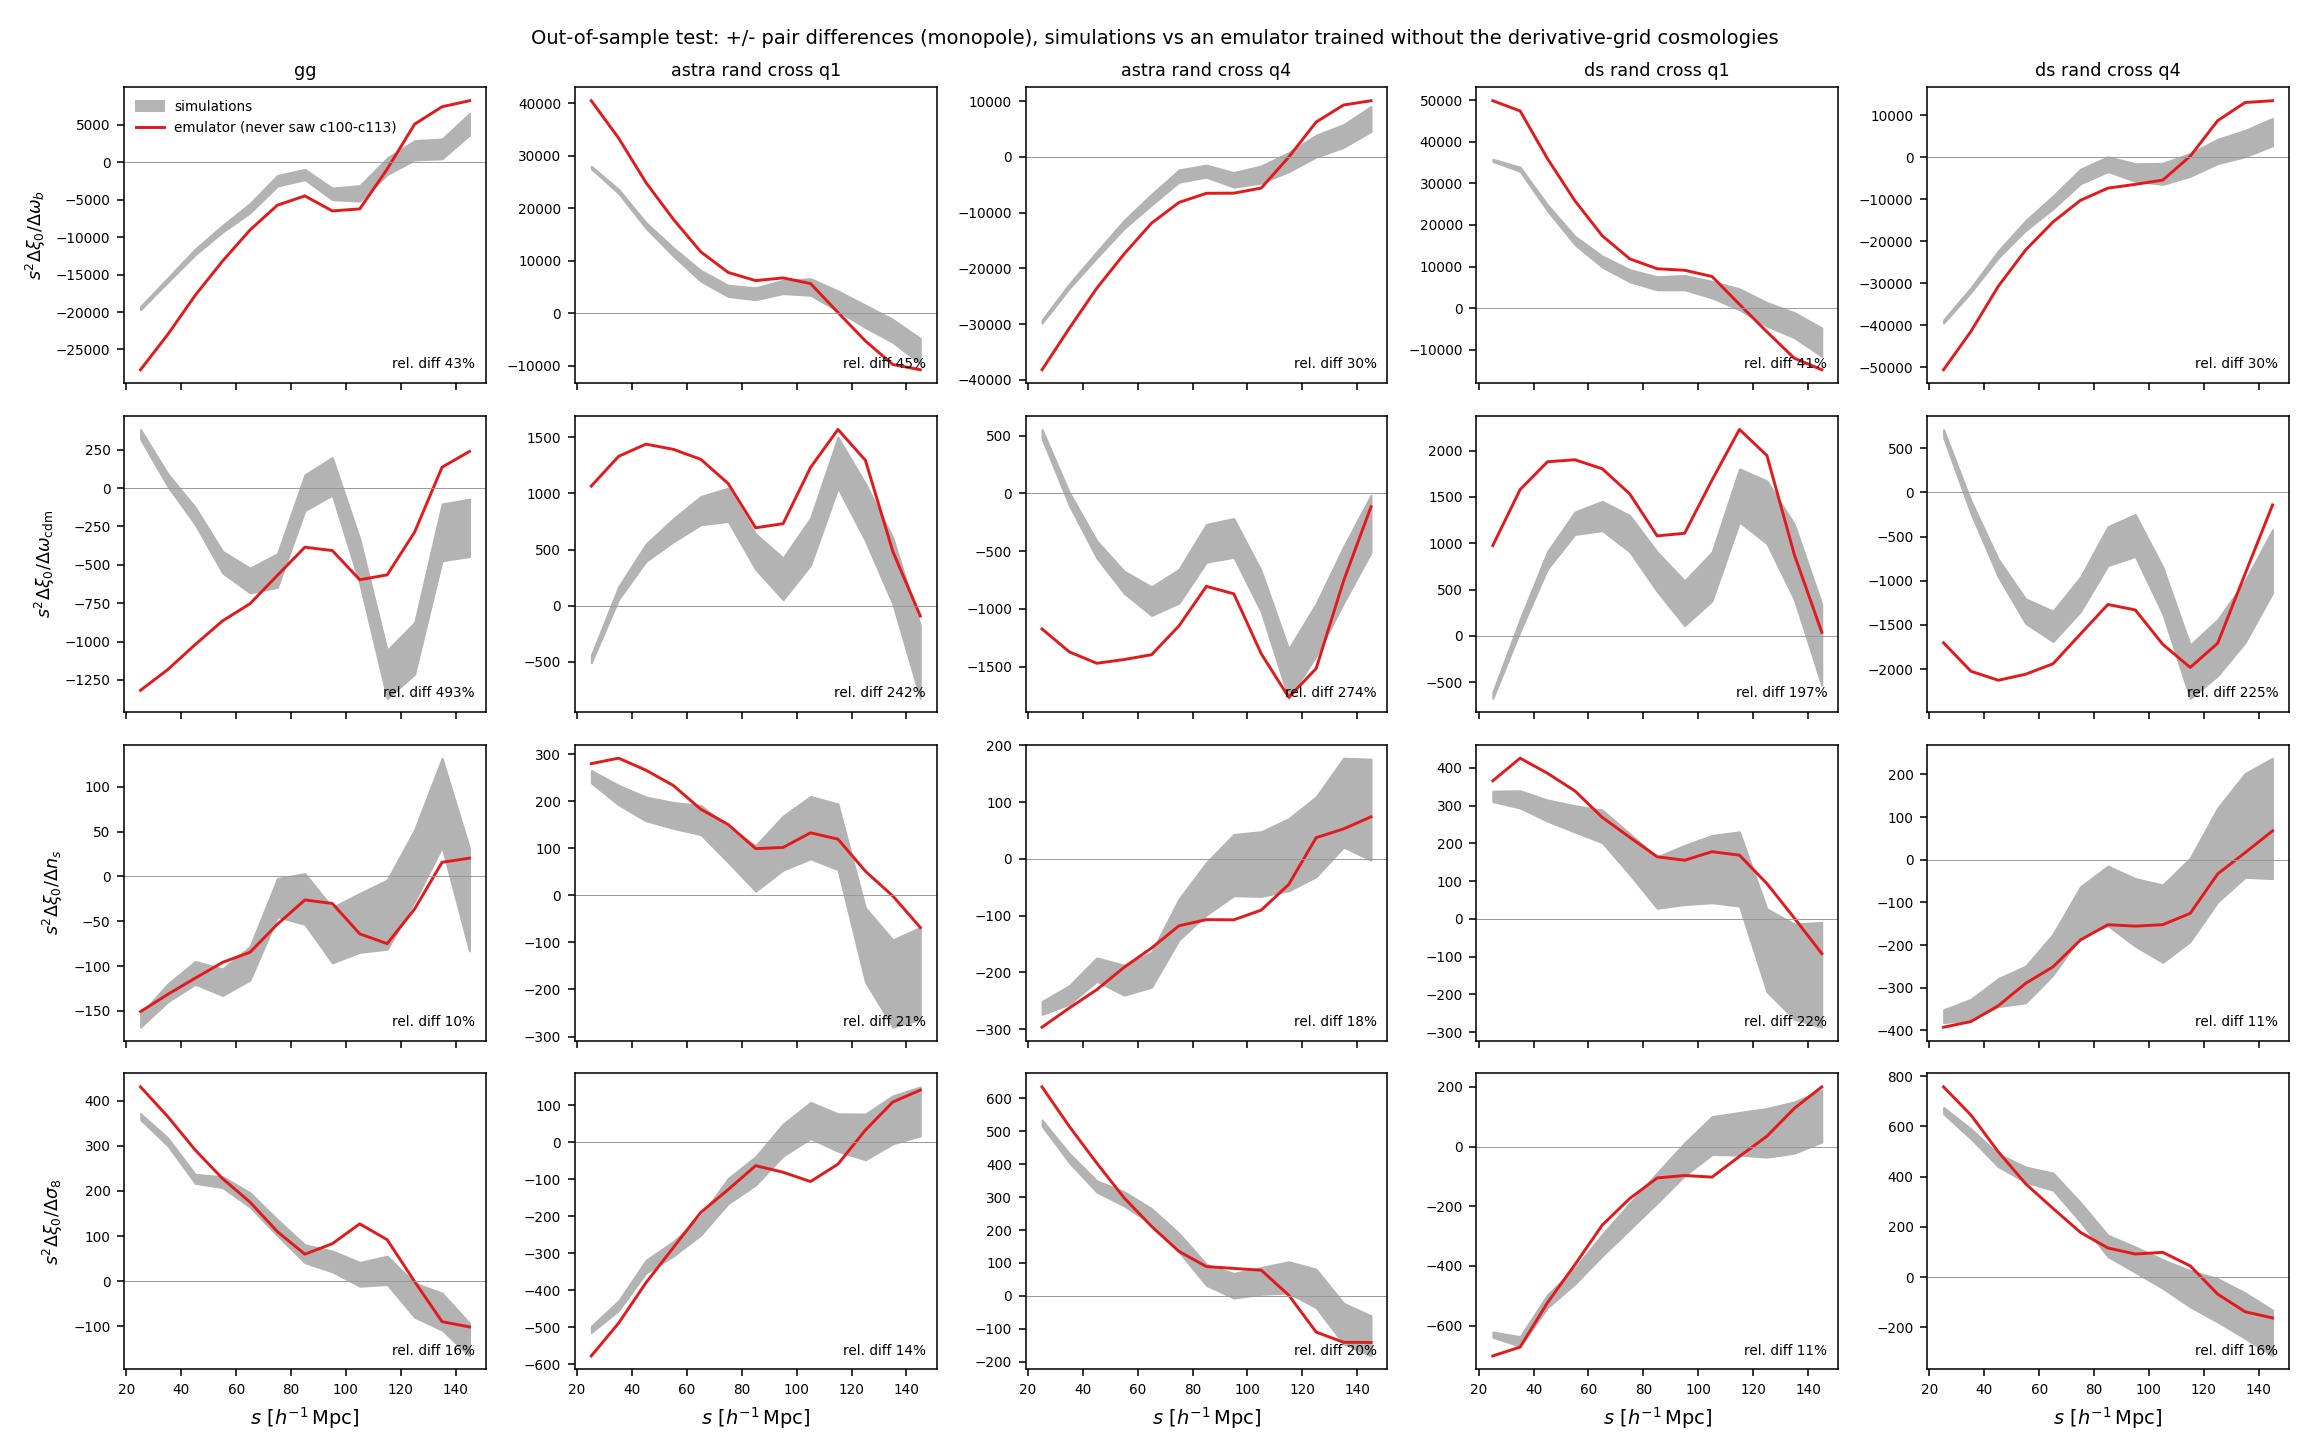
\includegraphics[width=\textwidth]{v2_derivatives_loco.png}
\caption{Test hors échantillon de la réponse cosmologique : monopôle des différences $\pm$ des paires dans les simulations (bande grise : moyenne $\pm$ erreur sur les 192 échantillons appariés) et prédit par un émulateur entraîné sans les cosmologies de la grille de dérivées (rouge).}
\label{fig:loco}
\end{figure*}

\begin{figure*}[!tp]
\centering
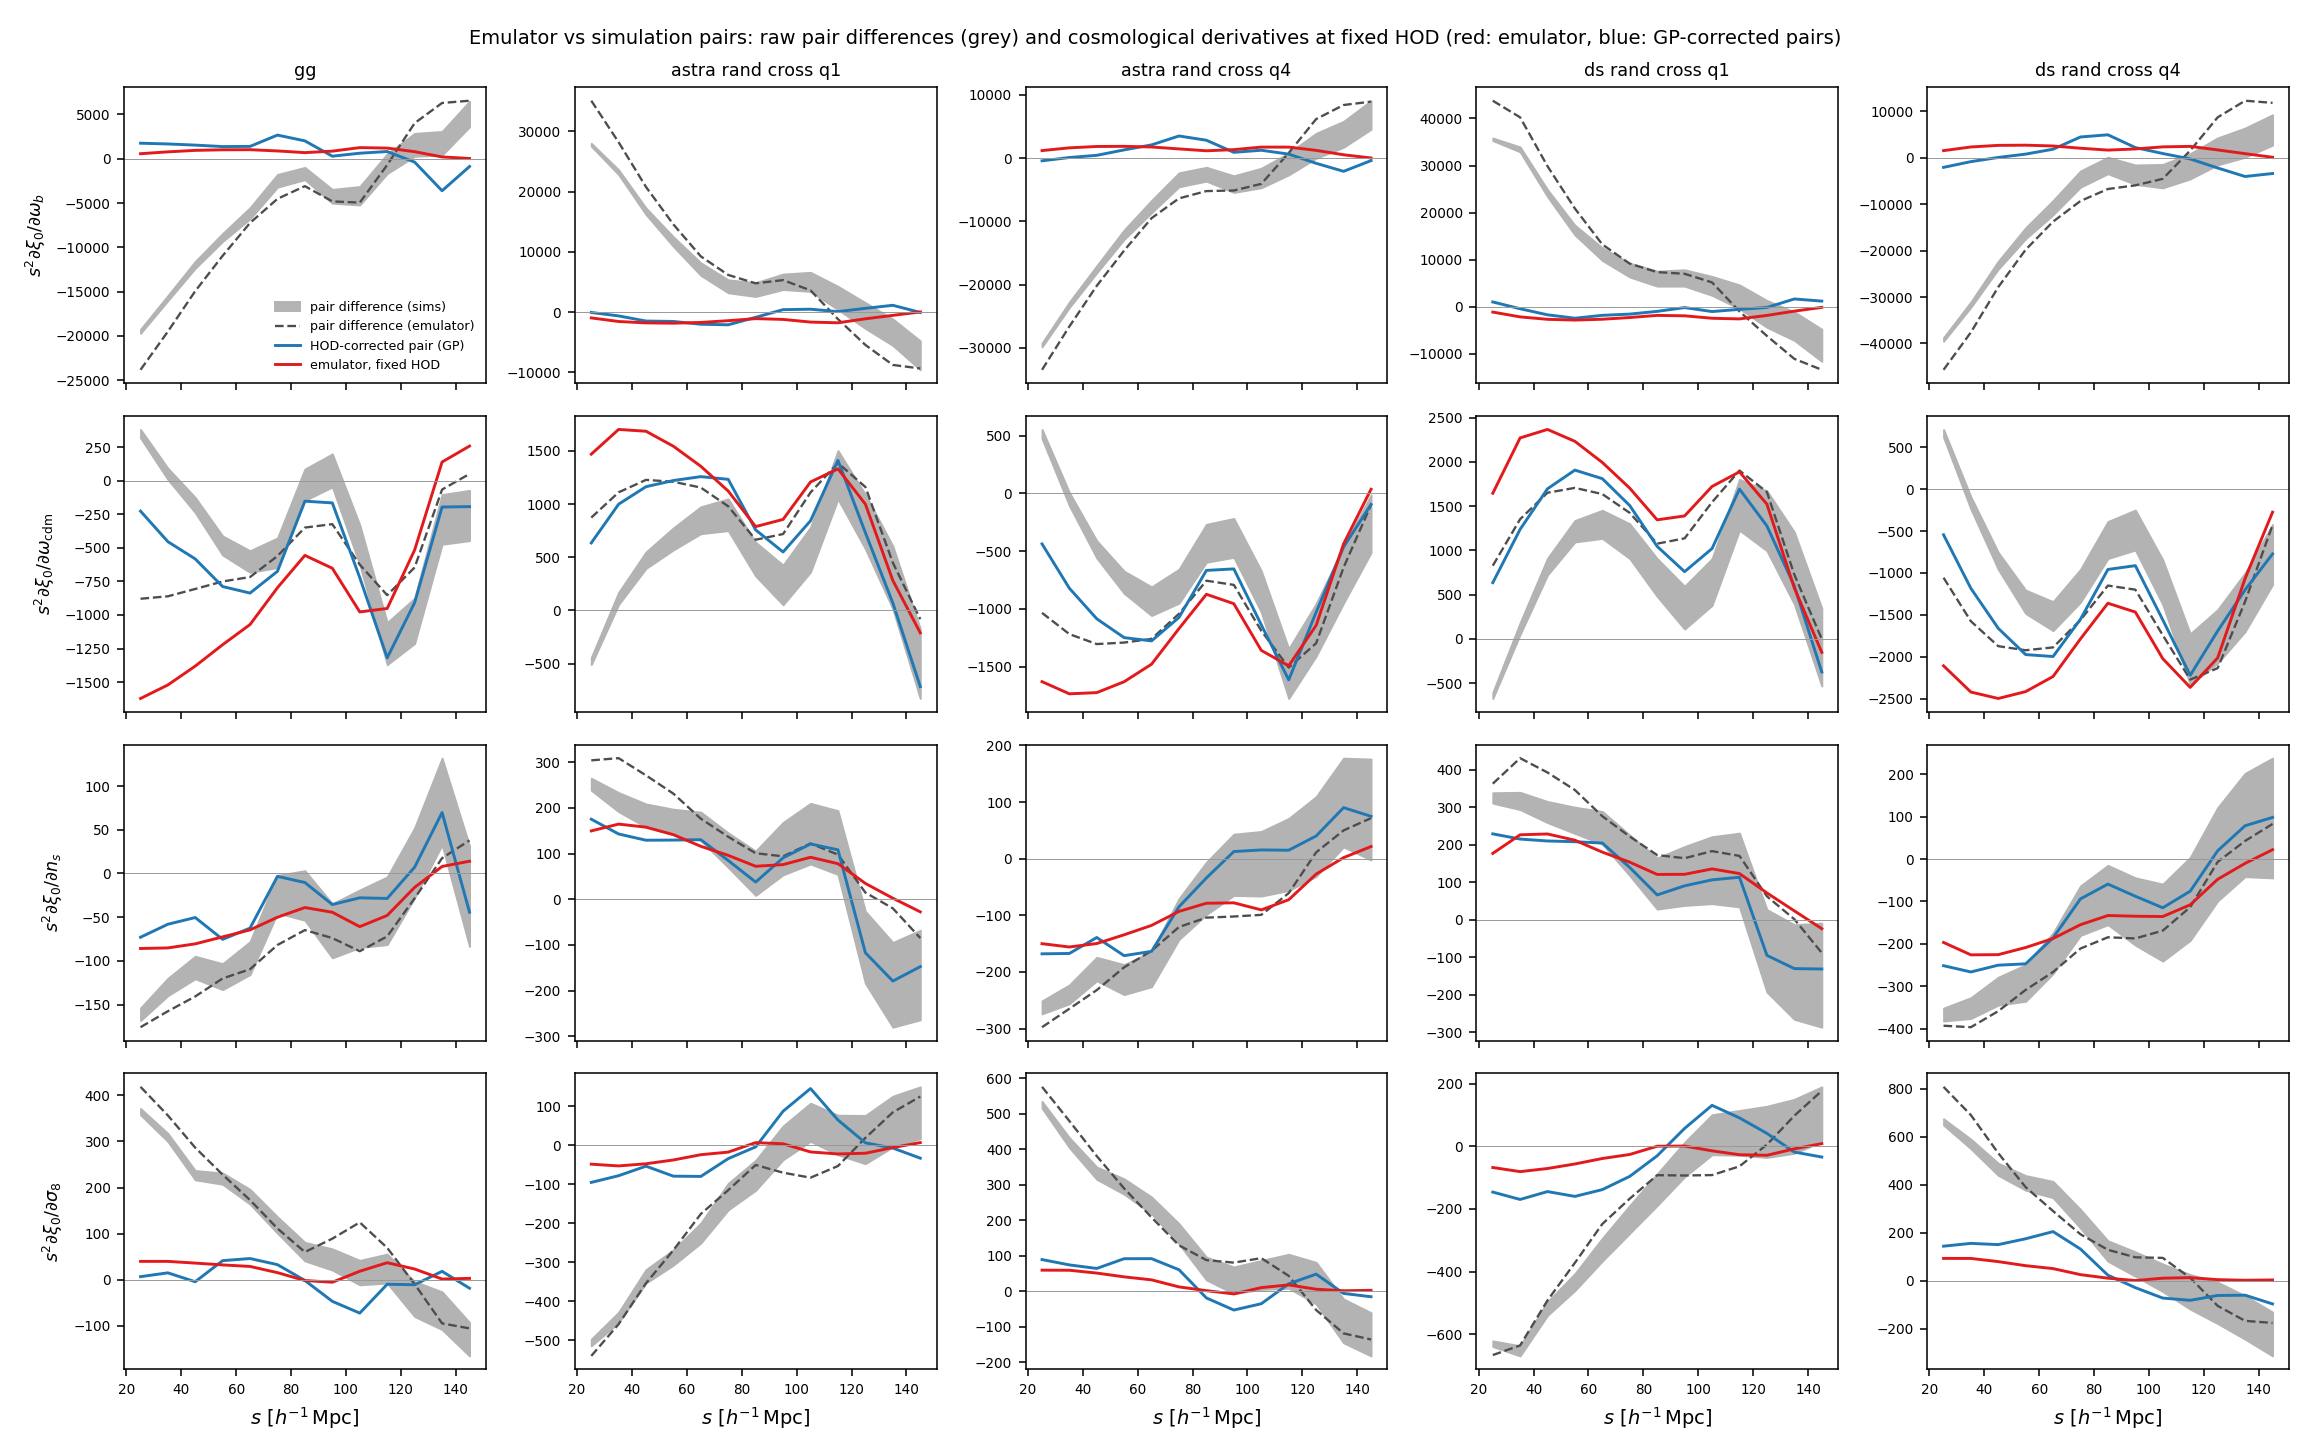
\includegraphics[width=\textwidth]{v2_emulator_vs_pairs.png}
\caption{Dérivées cosmologiques à HOD fixée issues de l'émulateur (rouge) et des différences de paires corrigées par la calibration GP de la réponse à la HOD (bleu), avec les différences brutes de paires dans les simulations (gris) et telles que prédites par l'émulateur (tirets).}
\label{fig:emu_pairs}
\end{figure*}

\begin{figure}[!htbp]
\centering
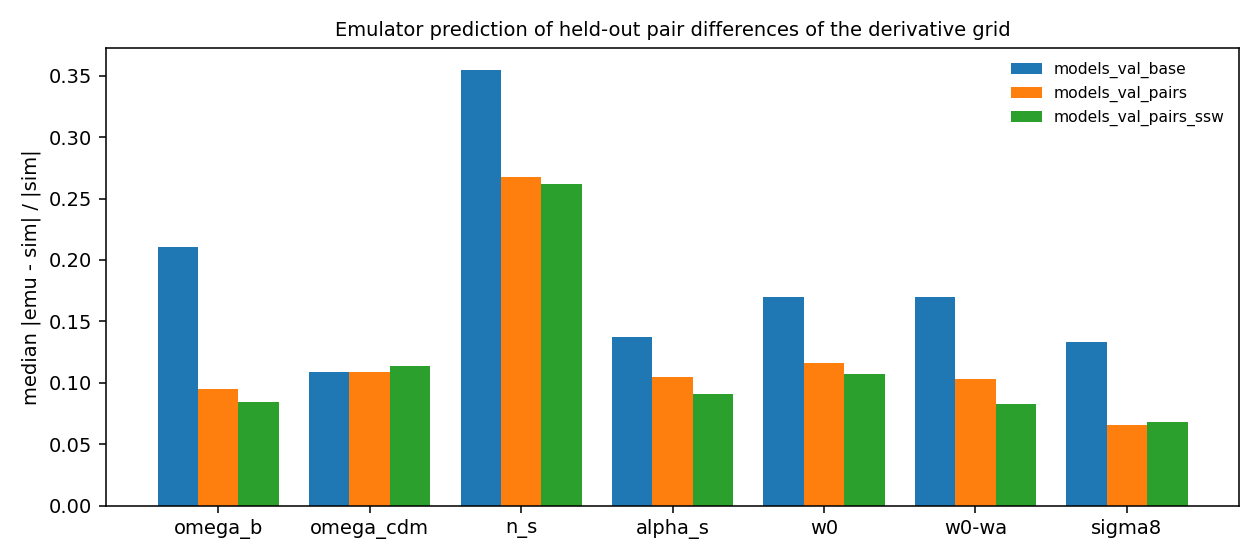
\includegraphics[width=\linewidth]{v2_validate_local.png}
\caption{Erreur relative médiane de la prédiction par l'émulateur des différences de paires exclues de la grille de dérivées, pour les trois variantes d'entraînement (Tableau~\ref{tab:local}).}
\label{fig:local}
\end{figure}

\begin{figure*}[!tp]
\centering
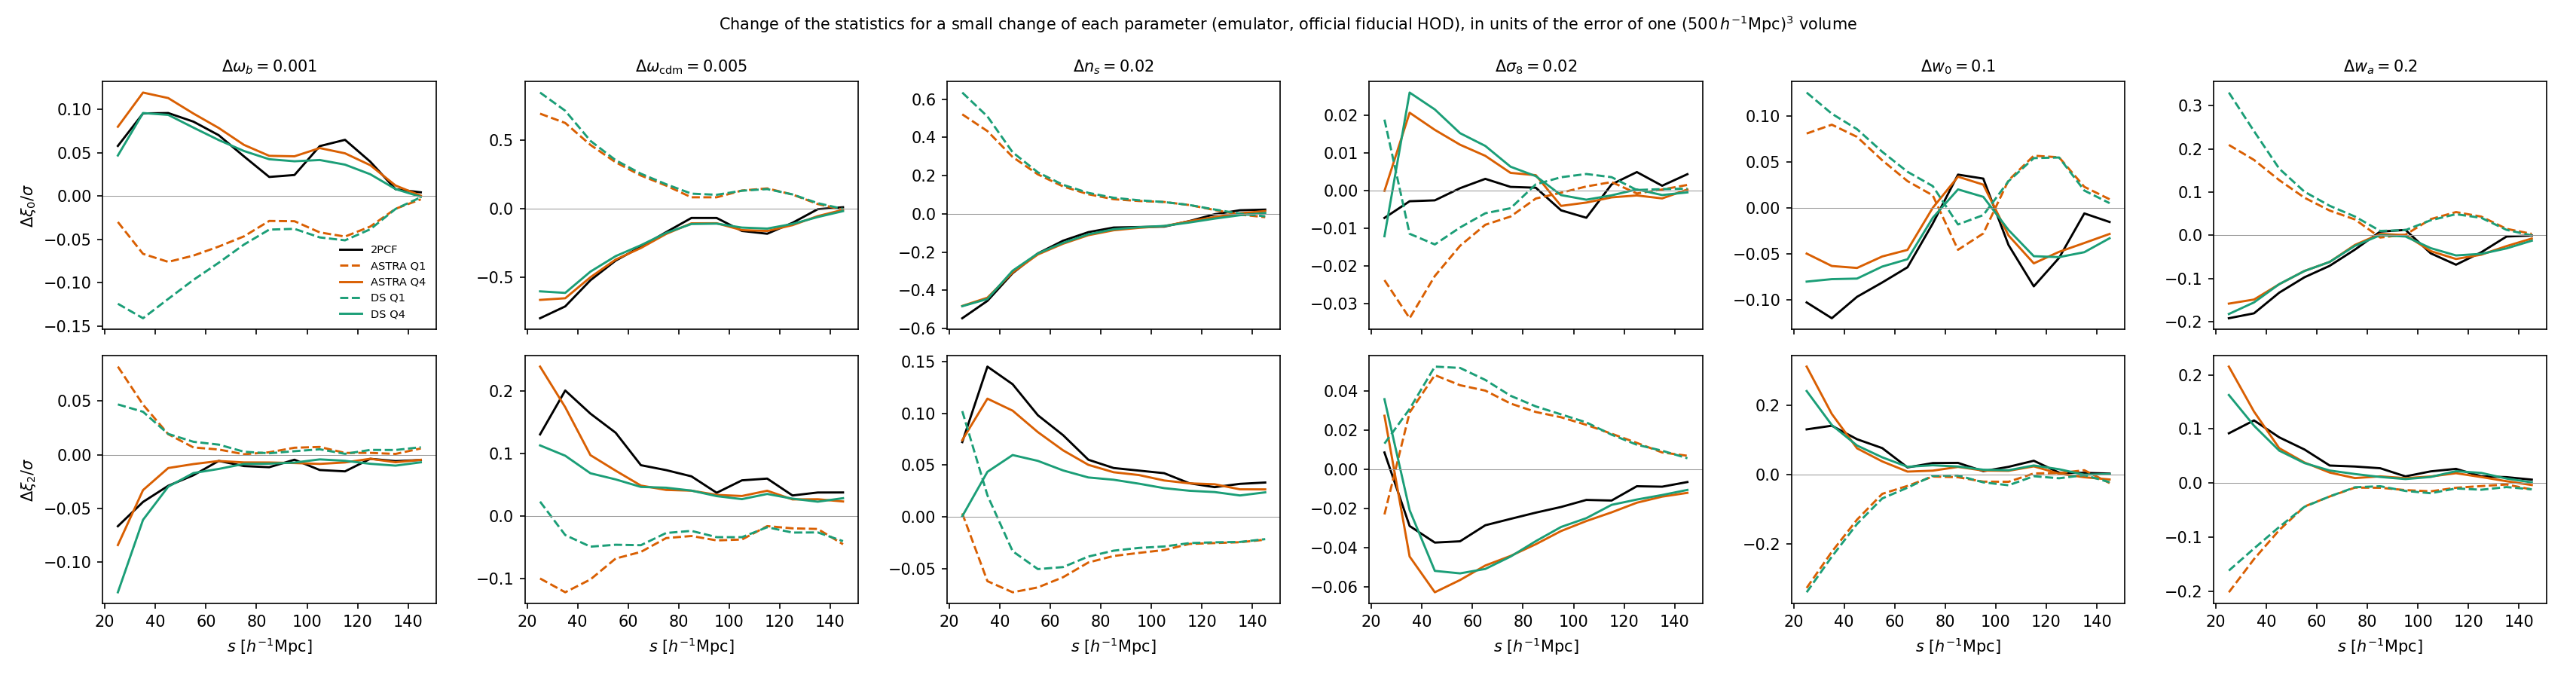
\includegraphics[width=\textwidth]{v2_derivatives.png}
\caption{Variation du monopôle (haut) et du quadrupôle (bas) pour un petit changement de chaque paramètre, en unités de l'erreur d'un volume de $(500\Mpch)^3$ (émulateur de référence au point fiduciel officiel) : 2PCF (noir), corrélations croisées Q1 (tirets) et Q4 (trait plein) de l'ASTRA split (orange) et du density split (vert).}
\label{fig:derivs}
\end{figure*}

\begin{figure}[!htbp]
\centering
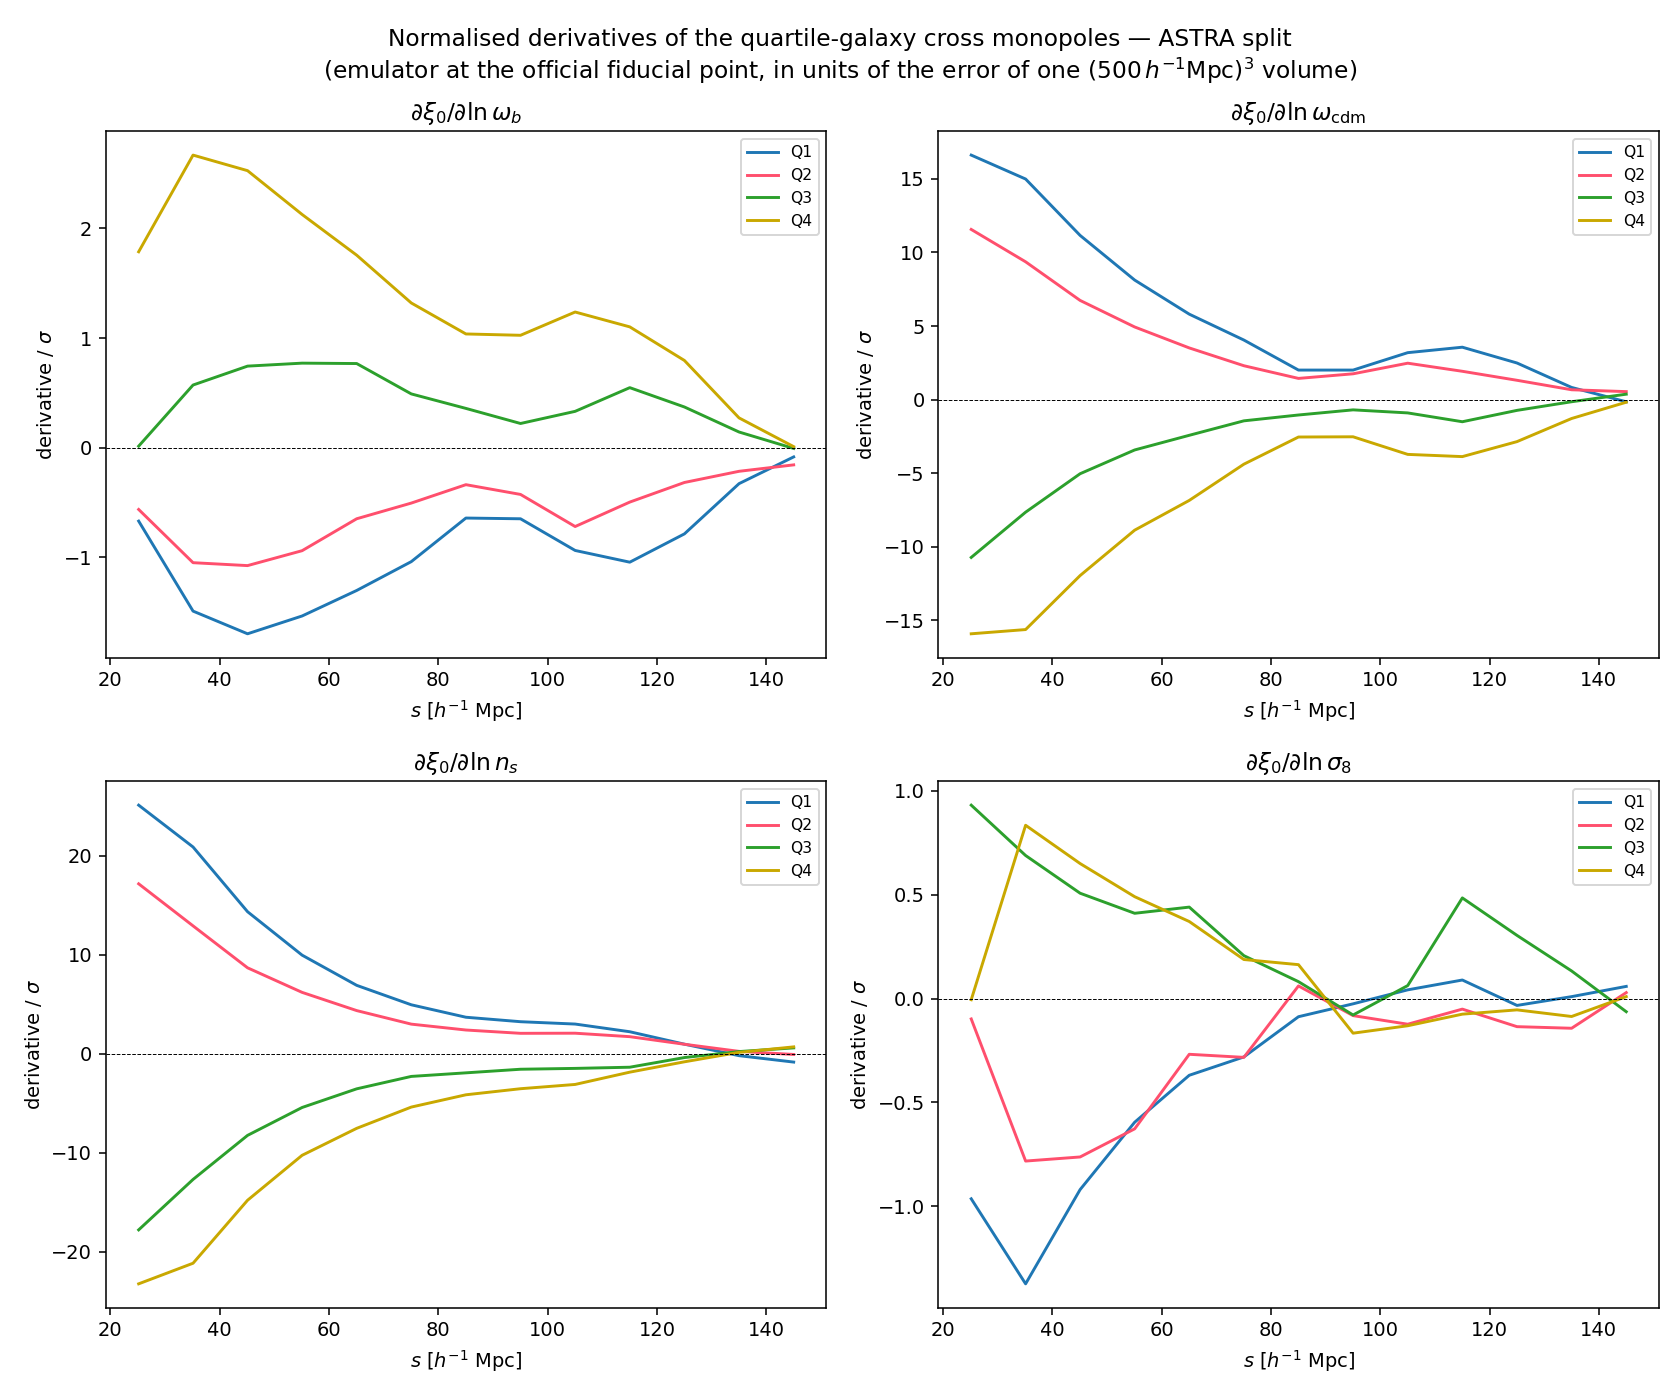
\includegraphics[width=\linewidth]{v1style_derivatives_astra.png}
\caption{ASTRA split : variation des quatre monopôles croisés quartile--galaxie pour un petit changement $\Delta\theta$ de chaque paramètre (valeur dans le titre de chaque panneau), en unités de l'erreur d'un volume de $(500\Mpch)^3$ (émulateur de référence, point fiduciel officiel).}
\label{fig:der_astra}
\end{figure}

\begin{figure}[!htbp]
\centering
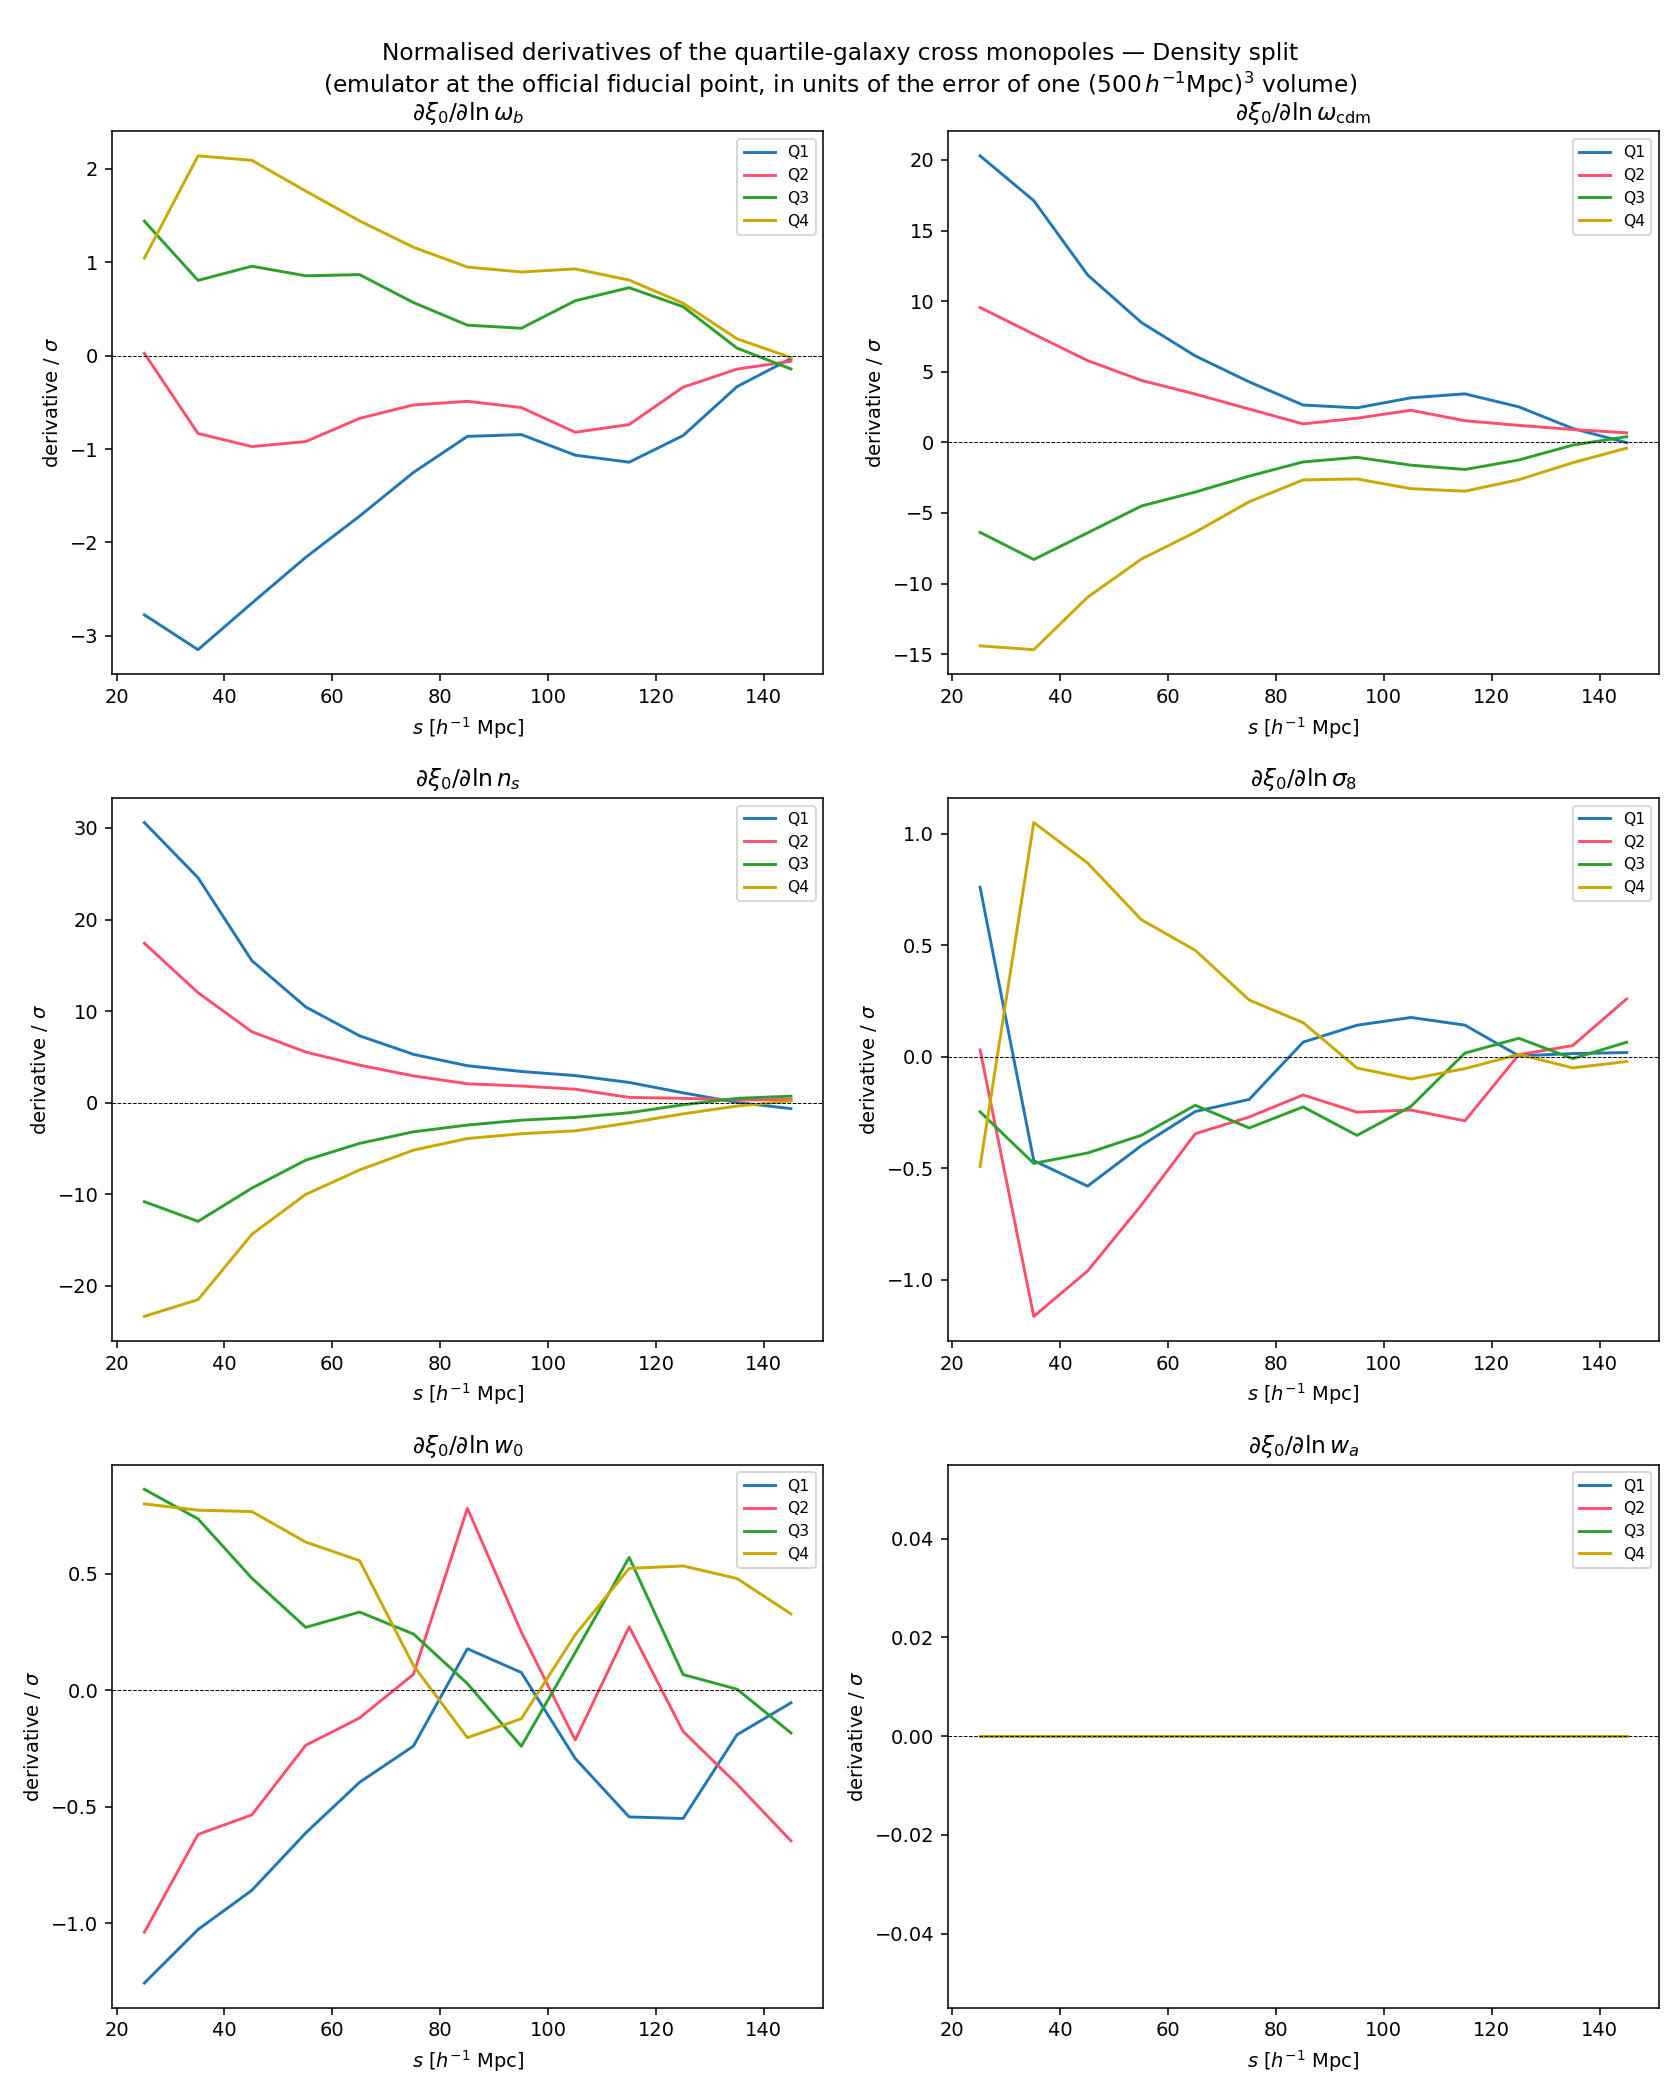
\includegraphics[width=\linewidth]{v1style_derivatives_ds.png}
\caption{Identique à la Figure~\ref{fig:der_astra} pour le density split.}
\label{fig:der_ds}
\end{figure}

\subsection{Dérivées par régression sur les paires}
\label{sec:regression}

Comme alternative à l'émulateur, nous estimons les dérivées localement à partir de la seule grille de dérivées. Pour une paire de cosmologies $c_\pm$, tous les catalogues de chaque cosmologie situés à une distance inférieure à $r_{\max}$ de la HOD fiducielle $h_0$ (les 16 tirages de la densification, le tirage de la paire et les tirages de l'émulateur) sont ajustés par un développement au premier ordre dans les paramètres de HOD, $\boldsymbol d_c(h) = \boldsymbol a_c + G\,(h-h_0)$, avec une réponse $G$ partagée par les deux cosmologies ; la dérivée est $(\boldsymbol a_{c_+}-\boldsymbol a_{c_-})/(\theta_+-\theta_-)$, la différence entre les deux cosmologies à la HOD exactement fiducielle. L'ajustement est effectué sous-volume par sous-volume : les catalogues des deux cosmologies partagent les mêmes conditions initiales, donc un même sous-volume contient les mêmes structures dans les deux, et leur différence est exempte de la majeure partie de la variance cosmique. Les erreurs sont obtenues par bootstrap des sous-volumes (réajustement sur des rééchantillonnages aléatoires de ceux-ci), ce qui propage la dispersion entre sous-volumes dans les dérivées. Les ordonnées à l'origine sont interpolées au milieu des tirages entourant $h_0$, et la courbure commune aux deux cosmologies s'annule dans la différence. Cet estimateur repose sur un modèle linéaire et sur la seule grille de dérivées, alors que l'émulateur est un modèle non linéaire de toute la suite : l'accord entre les deux est un test sévère des dérivées.

\paragraph{Espace de HOD réduit.} Avec 12 paramètres de HOD et $\sim18$ catalogues par cosmologie, l'ajustement est mal conditionné : il y a presque autant d'inconnues que de points de données, de sorte que l'ajustement peut reproduire les catalogues qui lui sont donnés mais pas en prédire de nouveaux. Son erreur leave-one-out (chaque catalogue étant prédit par un ajustement sur les autres) vaut 0.8--1.0 fois la dispersion entre HOD, c'est-à-dire que l'ajustement ne prédit guère mieux que la moyenne. C'est un problème classique de surajustement, résolu en réduisant le nombre de directions libres. Nous les déterminons indépendamment, à partir des 72 catalogues de calibration fiduciels : une décomposition en valeurs singulières de la réponse linéaire des statistiques à la HOD (chacune pondérée par son erreur statistique) donne les combinaisons de paramètres de HOD ordonnées selon l'ampleur de leur effet sur les statistiques. Les valeurs singulières sont $1, 0.054, 0.014, 0.013,\dots$ : \emph{les statistiques de clustering répondent essentiellement à une seule combinaison des 12 paramètres de HOD}, vraisemblablement le biais des galaxies à grande échelle, les autres étant 20 à 100 fois plus faibles. En conservant 3 ou 4 directions, l'erreur leave-one-out tombe à 0.7--0.9 fois la dispersion de la HOD, au niveau du bruit de mesure, et les deux choix donnent les mêmes prévisions à 5\% près. Nous utilisons 3 directions.

\subsection{Matrices de Fisher}
\label{sec:fishermat}

Les dérivées $D=\partial\boldsymbol d/\partial(\boldsymbol\theta,\boldsymbol h)$ sont obtenues au point fiduciel pour les 6 paramètres cosmologiques $\boldsymbol\theta=(\omega_b,\omega_{\rm cdm},n_s,\sigma_8,w_0,w_a)$ et les 12 paramètres de HOD $\boldsymbol h$. La covariance est la somme de la covariance mesurée et de l'erreur (diagonale) de l'émulateur : l'erreur de l'émulateur est une incertitude supplémentaire sur le modèle, indépendante des fluctuations statistiques des données, et des incertitudes indépendantes s'ajoutent en variance. La matrice de Fisher $F = D^T\hat C^{-1}D + P_h$ inclut un prior gaussien $P_h$ sur les paramètres de HOD de largeur 0.29 fois l'étendue du prior (l'écart-type du prior uniforme) ; les erreurs cosmologiques sont marginalisées sur la HOD en inversant la matrice complète $18\times18$, et nous donnons aussi les erreurs à HOD fixée. La marginalisation sur la HOD dégrade les contraintes de moins de $\sim30\%$, le paramètre le plus affecté étant $n_s$ : les paramètres de HOD miment en partie l'effet des paramètres cosmologiques (par exemple, un changement de biais des galaxies change l'amplitude du clustering comme $\sigma_8$), et les laisser libres absorbe une partie du signal cosmologique ; la faible dégradation montre que les statistiques distinguent bien la cosmologie de la formation des galaxies. L'incertitude due à l'entraînement de l'émulateur est estimée à partir de la dispersion des prévisions des réseaux individuels, divisée par $\sqrt{10}$.

\paragraph{Compression.} Chaque vecteur de données est comprimé en un nombre par paramètre (18 nombres), $\boldsymbol t=W^T\boldsymbol d$, $W=\tilde C^{-1}D$ ($\tilde C$ : estimation de la covariance par rétrécissement de Ledoit--Wolf), dont la covariance est ensuite estimée à partir des échantillons (facteur de Hartlap 0.90 avec 192 échantillons, 0.99 avec 1786). La compression est sans perte si $\tilde C=C$ ; sinon elle conserve moins d'information, ce qui rend les erreurs de prévision plus grandes, jamais plus petites, car la matrice de Fisher de $\boldsymbol t$ est calculée exactement avec sa propre covariance (Annexe~\ref{app:maths}) ; elle permet de comparer équitablement des vecteurs de données longs et combinés.
